\documentclass[a4paper,12pt]{article}
\usepackage[margin=1in]{geometry}
\usepackage{graphicx}
\usepackage{listings}
\usepackage{xcolor}

\title{Lab 3: MPI File Transfer}
\author{}
\date{}

\lstset{
    basicstyle=\ttfamily\footnotesize,
    numbers=left,
    numberstyle=\tiny,
    stepnumber=1,
    breaklines=true,
    frame=single,
    rulecolor=\color{black},
    keywordstyle=\color{blue},
    commentstyle=\color{green},
    stringstyle=\color{red},
}

\begin{document}

\maketitle

\section*{1. Rationale for MPI Implementation}
We chose **mpi4py** for its efficient integration of the Message Passing Interface (MPI) with Python. It offers straightforward APIs for parallel communication, supports essential MPI features (e.g., point-to-point messaging), and is compatible with widely used MPI distributions such as MPICH and OpenMPI. This combination of flexibility and performance makes mpi4py an ideal choice for our file transfer system.

\section*{2. System Design}
The system is composed of two main processes: the client (Rank 0) and the server (Rank 1). The client reads the file in chunks and transmits them to the server, which reconstructs the file and writes it to disk. Communication is facilitated via **MPI\_COMM\_WORLD**, with unique message tags used to identify data types.

\noindent \textbf{Figure: MPI File Transfer Architecture}
\begin{figure}[h!]
    \centering
    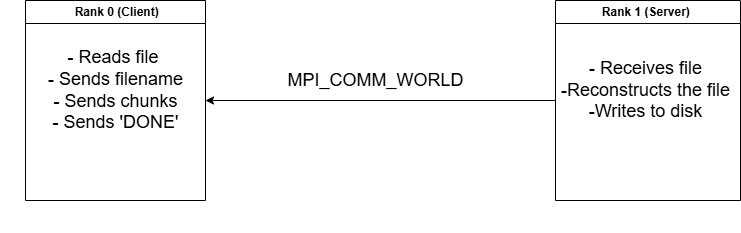
\includegraphics[width=0.8\textwidth]{design.png} % Replace with your image path
    \caption{Architecture of the MPI File Transfer System}
\end{figure}

\section*{3. Workflow and Process Description}
The workflow is divided into two distinct processes:

\subsection*{3.1 Client Process (Rank 0)}
\begin{itemize}
    \item Reads the file from the local system in chunks of 1 KB.
    \item Sends the file name to the server, followed by the file data in chunks.
    \item Signals the end of the transfer using a termination message (`DONE`).
\end{itemize}

\subsection*{3.2 Server Process (Rank 1)}
\begin{itemize}
    \item Receives the file name from the client and prepares to write to disk.
    \item Collects file chunks and reconstructs the file.
    \item Completes the transfer when the termination message (`DONE`) is received.
\end{itemize}

\noindent \textbf{Figure: Data Flow in the MPI Service}
\begin{figure}[h!]
    \centering
    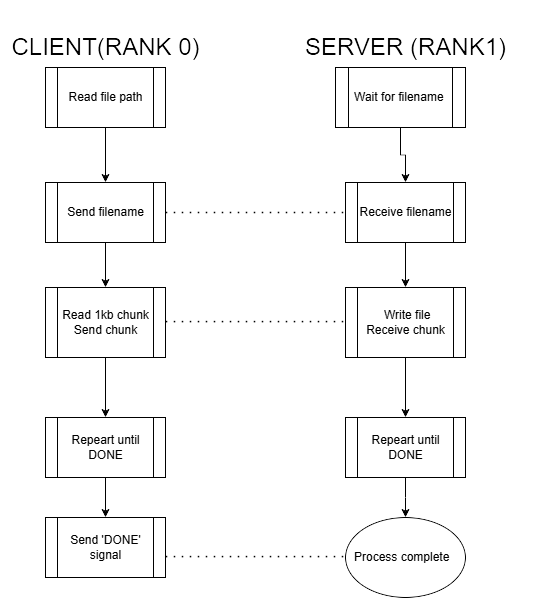
\includegraphics[width=0.8\textwidth]{implement_flow.png} % Replace with your image path
    \caption{MPI Data Flow and Communication}
\end{figure}

\section*{4. Implementation Summary}
\subsection*{4.1 Client Implementation}
The client opens the specified file, reads it in 1 KB chunks, and sends the data to the server via `comm.send()`. After all chunks are sent, it transmits a `DONE` signal to indicate the transfer is complete.

\subsection*{4.2 Server Implementation}
The server listens for incoming messages from the client. It receives the file name first, followed by the data chunks. The chunks are written sequentially to reconstruct the file. The process ends upon receiving the `DONE` signal.

\section*{5. Task Allocation and Contributions}
\begin{itemize}
    \item **Research on MPI and mpi4py**: Cao Nhat Nam (22BI13320) and Pham Ngoc Minh Chau (22BI13063)
    \item **Client-Side and Server-Side Code Development**: Do Thi Huong Tra (BA12-174)
    \item **Testing and Debugging**: Vu Hoang Mai Nhi (22BI13352)
    \item **Report Writing and Diagrams**: Bui Nguyen Ngoc Huyen (22BI13199)
\end{itemize}

\end{document}
